\documentclass{beamer}
\usepackage[utf8]{inputenc}

\usetheme{Madrid}
\usecolortheme{default}
\usepackage{amsmath,amssymb,amsfonts,amsthm}
\usepackage{txfonts}
\usepackage{tkz-euclide}
\usepackage{listings}
\usepackage{adjustbox}
\usepackage{array}
\usepackage{tabularx}
\usepackage{gvv}
\usepackage{lmodern}
\usepackage{circuitikz}
\usepackage{tikz}
\usepackage{graphicx}
\usepackage{mathtools}
\setbeamertemplate{page number in head/foot}[totalframenumber]

\usepackage{tcolorbox}
\tcbuselibrary{minted,breakable,xparse,skins}



\definecolor{bg}{gray}{0.95}
\DeclareTCBListing{mintedbox}{O{}m!O{}}{%
  breakable=true,
  listing engine=minted,
  listing only,
  minted language=#2,
  minted style=default,
  minted options={%
    linenos,
    gobble=0,
    breaklines=true,
    breakafter=,,
    fontsize=\small,
    numbersep=8pt,
    #1},
  boxsep=0pt,
  left skip=0pt,
  right skip=0pt,
  left=25pt,
  right=0pt,
  top=3pt,
  bottom=3pt,
  arc=5pt,
  leftrule=0pt,
  rightrule=0pt,
  bottomrule=2pt,
  toprule=2pt,
  colback=bg,
  colframe=orange!70,
  enhanced,
  overlay={%
    \begin{tcbclipinterior}
    \fill[orange!20!white] (frame.south west) rectangle ([xshift=20pt]frame.north west);
    \end{tcbclipinterior}},
  #3,
}
\lstset{
    language=C,
    basicstyle=\ttfamily\small,
    keywordstyle=\color{blue},
    stringstyle=\color{orange},
    commentstyle=\color{green!60!black},
    numbers=left,
    numberstyle=\tiny\color{gray},
    breaklines=true,
    showstringspaces=false,
}

\title 
{3.2.3}
\date{September 14, 2025}


\author 
{Vivek K Kumar - EE25BTECH11062}



\begin{document}


\frame{\titlepage}
\begin{frame}{Question}
Draw a parallelogram ABCD in which $BC = 5cm, AB = 3cm$ and $\angle ABC = 60^\circ $, divide it into triangles ACB and ABD by the diagonal BD
\end{frame}

\begin{frame}{Solution}
Let $\vec{A}$, $\vec{B}$, $\vec{C}$ and $\vec{D}$ represent position vectors of the vertices of parallelogram.

Given information, 
\begin{align}
\norm{\vec{A-B}} &= 3 \\
\norm{\vec{C-B}} &= 5 \\
\angle B &= \frac{\pi}{3}
\end{align}
The coordinates of $\vec{A}, \vec{B}, \vec{C}$ can be expressed as
\begin{align}
\vec{B} &= \myvec{0\\0} \\
\vec{C} &= \norm{\vec{C-B}}\myvec{1\\0} \\
\vec{A} &= \norm{\vec{A-B}}\myvec{cosB\\sinB} 
\end{align}
\end{frame}
\begin{frame}{Solution}
Since $\vec{A}, \vec{B}, \vec{C}, \vec{D}$ form vertices of a parallelogram,
\begin{align}
\frac{\vec{A}+\vec{C}}{2} &= \frac{\vec{B}+\vec{D}}{2} \\
\vec{D} &= \vec{A+C-B}\\
\vec{D} = \norm{\vec{A}-\vec{B}}\myvec{cosB\\sinB} &+  \norm{\vec{C}-\vec{B}}\myvec{1\\0} - \myvec{0\\0}
\end{align}
Substituting values, 
\begin{align}
    \vec{A} &= \myvec{3/2 \\ 3\sqrt{3}/{2}} \\
    \vec{B} &= \myvec{0 \\ 0} \\
    \vec{C} &= \myvec{5 \\ 0}
\end{align}
\end{frame}

\begin{frame}{Variables used}
\begin{align}
\vec{D} &= \myvec{13/2 \\ 3\sqrt{3}/2}
\end{align}
\begin{table}[H]    
  \centering
  \begin{tabular}{|c|c|}
\hline
\textbf{Name} & \textbf{Value} \\ \hline
$\vec{A}$ & $\myvec{2 & 1 \\0 & 3}$ \\ \hline
\end{tabular}

  \caption{Coordinates of vertices of parallelogram}
  \label{tab:2.9.13}
\end{table}

\end{frame}

\begin{frame}[fragile]
    \frametitle{Python - Importing libraries and checking system}
    \begin{lstlisting}
import sys
import numpy as np
import numpy.linalg as LA
import matplotlib.pyplot as plt
import matplotlib.image as mpimg
import math

from libs.line.funcs import *
from libs.triangle.funcs import *
from libs.conics.funcs import circ_gen

import subprocess
import shlex

print('Using termux?(y/n)')
y = input()
\end{lstlisting}
\end{frame}

\begin{frame}[fragile]
    \frametitle{Python - Defining vertices of parallelogram}
    \begin{lstlisting}
A = np.array([3/2, 3*math.sqrt(3)/2]).reshape(-1, 1)
B = np.array([0, 0]).reshape(-1, 1)
C = np.array([5, 0]).reshape(-1, 1)
D = np.array([13/2, 3*math.sqrt(3)/2]).reshape(-1,1)
\end{lstlisting}
\end{frame}

\begin{frame}[fragile]
    \frametitle{Python - Generating points and plotting}
    \begin{lstlisting}
p_A = line_gen(A, B)
p_B = line_gen(B, C)
p_C = line_gen(C, D)
p_D = line_gen(D, A)
p_BD = line_gen(B, D)

fig = plt.figure()
ax = fig.add_subplot(111)
ax.plot(p_A[0, :], p_A[1, :], label = 'Line AB')
ax.plot(p_B[0, :], p_B[1, :], label = 'Line BC')
ax.plot(p_C[0, :], p_C[1, :], label = 'Line CD')
ax.plot(p_D[0, :], p_D[1, :], label = 'Line DA')
ax.plot(p_BD[0, :], p_BD[1, :], label = 'Line BD')
\end{lstlisting}
\end{frame}

\begin{frame}[fragile]
    \frametitle{Python - Labelling points}
    \begin{lstlisting}
pts = np.block([A, B, C, D])
names = ['A', 'B', 'C', 'D']
for i in range(4):
    X = pts[:, i]
    ax.text(X[0], X[1], s=f'{names[i]}({round(X[0], 3)}, {round(X[1],3)})')

ax.set_xlabel('$x$')
ax.set_ylabel('$y$')
ax.legend(loc='best')
ax.grid(True) 
ax.axis('equal')
ax.set_xlim([-5, 10])
ax.set_ylim([-5, 10])
    \end{lstlisting}
\end{frame}

\begin{frame}[fragile]
    \frametitle{Python - Saving figure and opening it}
    \begin{lstlisting}
fig.savefig('../figs/fig.png')
print('Saved figure to ../figs/fig.png')

if(y == 'y'):
    subprocess.run(shlex.split('termux-open ../figs/fig.png'))
else:
    subprocess.run(["open",  "../figs/fig.png"])
    \end{lstlisting}
\end{frame}


\begin{frame}{Plot-Using only Python}
    \centering
    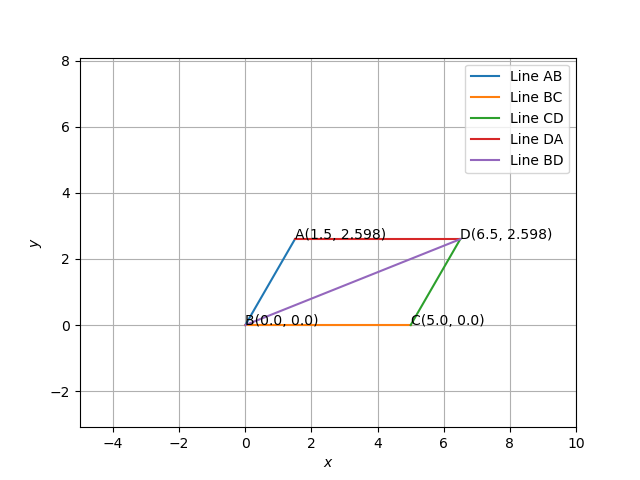
\includegraphics[width=\columnwidth, height=0.8\textheight, keepaspectratio]{../figs/fig.png}     
\end{frame}

\begin{frame}[fragile]
    \frametitle{C Code (0) - Importing libraries}

    \begin{lstlisting}
#include <stdio.h>
#include <stdlib.h>
#include <string.h>
#include <math.h>
#include <sys/socket.h>
#include <netinet/in.h>
#include <unistd.h>
#include "libs/matfun.h"
#include "libs/geofun.h"
    \end{lstlisting}
\end{frame}
\begin{frame}[fragile]
    \frametitle{C Code (1) - Function to Generate Points on a Line}

    \begin{lstlisting}

void point_gen(FILE *p_file, double **A, double **B, int rows, int cols, int npts){
    for(int i = 0; i <= npts; i++){
     double **output = Matadd(A, Matscale(Matsub(B, A, rows, cols), rows, cols, (double)i/npts), rows, cols);
     fprintf(p_file, "%lf, %lf\n", output[0][0], output[1][0]);
     freeMat(output, rows);
    }
}

    \end{lstlisting}
\end{frame}


\begin{frame}[fragile]
    \frametitle{C Code (2) - Function to write points b/w given point and origin to a file}

    \begin{lstlisting}
void write_points(double x1, double y1, double x2, double y2, double x3, double y3, double x4, double y4, int npts){
    int m = 2;
    int n = 1;

    double **A = createMat(m, n);
    double **B = createMat(m, n);
    double **C = createMat(m, n);
    double **D = createMat(m, n);

    B[0][0] = x2;
    B[1][0] = y2;
    \end{lstlisting}
\end{frame}
\begin{frame}[fragile]
    \frametitle{C Code (2) - Function to write points b/w given 2 points to a file}

    \begin{lstlisting}
    A[0][0] = x1;
    A[1][0] = y1;

    C[0][0] = x3;
    C[1][0] = y3;

    D[0][0] = x4;
    D[1][0] = y4;

    FILE *p_file;
    p_file = fopen("plot.dat", "w");
    if(p_file == NULL)
        printf("Error opening one of the data files\n");
    \end{lstlisting}
\end{frame}

\begin{frame}[fragile]
    \frametitle{C Code (2) - Function to write points b/w given 2 points to a file}
    \begin{lstlisting}
    point_gen(p_file, A, B, m, n, npts);
    point_gen(p_file, B, C, m, n, npts);
    point_gen(p_file, C, D, m, n, npts);
    point_gen(p_file, D, A, m, n, npts);
    point_gen(p_file, B, D, m, n, npts);

    freeMat(A, m);
    freeMat(B, m);
    freeMat(C, m);
    freeMat(D, m);

    fclose(p_file);
}
    \end{lstlisting}
\end{frame}

\begin{frame}[fragile]
    \frametitle{Python Code (0) - Importing libraries and checking system}
    \begin{lstlisting}
import numpy as np
import matplotlib.pyplot as plt
import ctypes
import os
import sys
import subprocess
import math

print('Using termux? (y/n)')
termux = input()
\end{lstlisting}
\end{frame}

\begin{frame}[fragile]
    \frametitle{Python Code (1) - Using Shared Object}
    \begin{lstlisting}
lib_path = os.path.join(os.path.dirname(__file__), 'plot.so')
my_lib = ctypes.CDLL(lib_path)

my_lib.write_points.argtypes = [ctypes.c_double, ctypes.c_double, ctypes.c_double, ctypes.c_double, ctypes.c_double, ctypes.c_double, ctypes.c_double, ctypes.c_double, ctypes.c_int]
my_lib.write_points.restype = None
A = np.array([3/2, 3*math.sqrt(3)/2]).reshape(-1, 1)
B = np.array([0, 0]).reshape(-1, 1)
C = np.array([5, 0]).reshape(-1, 1)
D = np.array([13/2, 3*math.sqrt(3)/2]).reshape(-1, 1)
npts = 20000
\end{lstlisting}
\end{frame}

\begin{frame}[fragile]
    \frametitle{Python Code (2) - Loading points and plotting them}
    \begin{lstlisting}
my_lib.write_points(A[0][0], A[1][0], B[0][0], B[1][0], C[0][0], C[1][0], D[0][0], D[1][0], npts)

fig = plt.figure()
ax = fig.add_subplot(111)
labels = ['AB', 'BC', 'CD', 'DA', 'BD']
pts = np.block([A, B, C, D])
vertices = ['A', 'B', 'C', 'D']
for i,label in enumerate(labels):
    points = np.loadtxt('plot.dat', delimiter = ',', usecols=(0,1))[i*(npts+1):(i+1)*(npts+1)]
    ax.plot(points[:, 0], points[:, 1], label = f'Line {label}')
    if(i<4):
        ax.text(pts[:, i][0], pts[:, i][1], s=f'{vertices[i]}({round(pts[:, i][0],3)}, {round(pts[:, i][1],3)})')
\end{lstlisting}
\end{frame}

\begin{frame}[fragile]
    \frametitle{Python Code (3) - Labelling plot}
    \begin{lstlisting}
        ax.set_xlabel('$x$')
        ax.set_ylabel('$y$')
        ax.legend(loc='best')
        ax.grid() 
        ax.axis('equal')
        ax.set_xlim([-5, 10])
        ax.set_ylim([-5, 10])
    \end{lstlisting}
\end{frame}

\begin{frame}[fragile]
    \frametitle{Python Code (4) - Saving and displaying plot}
    \begin{lstlisting}
fig.savefig('../figs/fig2.png')
print('Saved figure to ../figs/fig2.png')

if(termux == 'y'):
    subprocess.run(shlex.split('termux-open ../figs/fig2.png'))
else:
    subprocess.run(["open",  "../figs/fig2.png"])
\end{lstlisting}
\end{frame}

\begin{frame}{Plot-Using Both C and Python}
    \centering
    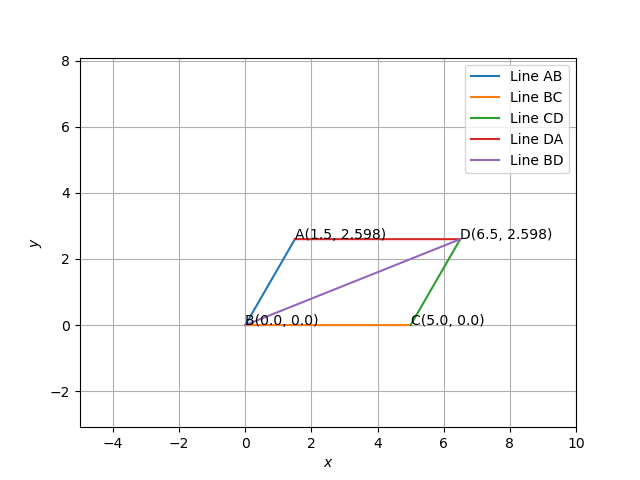
\includegraphics[width=\columnwidth, height=0.8\textheight, keepaspectratio]{../figs/fig2.png}     
\end{frame}

\end{document}
